\documentclass[uplatex,dvipdfmx]{jsarticle}
\usepackage{amssymb}
\usepackage{amsmath}
\usepackage{amsthm}
\usepackage{framed}
\usepackage{braket}
\usepackage{bm}
\usepackage{mathrsfs}
\usepackage{mathabx}
\usepackage{accents}
\usepackage{tocloft}
\usepackage[dvipdfmx]{graphicx}
\usepackage{tikz}
\usepackage{url}
\usepackage{color}
\usepackage{xifthen}
\usepackage{xcolor}
\usepackage{framed}
\usepackage{mathtools}
\usepackage[explicit]{titlesec}
\usepackage[normalem]{ulem}
\usepackage{hyperref}
\usepackage{pxjahyper}
\usepackage[backend=biber,style=numeric,sorting=none,doi=false,isbn=false,url=false]{biblatex}
\addbibresource{bib.bib}

\usetikzlibrary{positioning}
\usetikzlibrary{calc}
\usetikzlibrary{decorations.pathreplacing}
\usetikzlibrary{cd}

\newcommand{\scrN}{\mathcal{N}}
\newcommand{\scrC}{\mathcal{C}}
\newcommand{\X}{\mathcal{X}}
\newcommand{\Y}{\mathcal{Y}}
\newcommand{\N}{\mathbb{N}}
\newcommand{\Z}{\mathbb{Z}}
\newcommand{\Q}{\mathbb{Q}}
\newcommand{\R}{\mathbb{R}}
\newcommand{\C}{\mathbb{C}}
\newcommand{\range}{\operatorname{ran}}
\newcommand{\dom}{\operatorname{dom}}
\newcommand{\append}{{}^\frown}
\newcommand{\boldsig}{\boldsymbol{\Sigma}}
\newcommand{\boldpi}{\boldsymbol{\Pi}}
\newcommand{\bolddelta}{\boldsymbol{\Delta}}
\newcommand{\Ordinals}{\mathrm{On}}
\renewcommand\emptyset{\varnothing}
\renewcommand\subset{\subseteq}
\newcommand\forces{\Vdash}
\newcommand\notforces{\nVdash}
\newcommand{\rank}{\operatorname{rank}}
\newcommand{\BW}{\operatorname{BW}}
\newcommand{\B}{\operatorname{B}}
\newcommand{\MON}{\operatorname{MON}}

\def\pair<#1>{\langle #1 \rangle}

\newcommand{\needtocheck}[1][]{%
	\ifthenelse{\equal{#1}{}}{%
		\textcolor{blue}{[要チェック]}%
	}{%
		\textcolor{blue}{[要チェック: #1]}%
	}%
}

\newcommand{\todo}[1][]{%
	\ifthenelse{\equal{#1}{}}{%
		\textcolor{red}{[TODO]}%
	}{%
		\textcolor{red}{[TODO: #1]}%
	}%
}

\theoremstyle{definition}
\newtheorem{thm}{定理}
\newtheorem*{thm*}{定理}
\newtheorem{defi}[thm]{定義}
\newtheorem*{defi*}{定義}
\newtheorem{lem}[thm]{補題}
\newtheorem*{lem*}{補題}
\newtheorem{fact}[thm]{事実}
\newtheorem*{fact*}{事実}
\newtheorem*{formula*}{公式}
\newtheorem{prop}[thm]{命題}
\newtheorem*{prop*}{命題}
\newtheorem{exm}[thm]{例}
\newtheorem*{exm*}{例}
\newtheorem{rmk}[thm]{注意}
\newtheorem*{rmk*}{注意}
\newtheorem{cor}[thm]{系}
\newtheorem*{cor*}{系}
\newtheorem*{notation*}{記法}
\renewcommand{\proofname}{証明}
\newenvironment{claim}[1]{\par\noindent\underline{主張:}\space#1}{}
\newenvironment{claimproof}[1]{\par\noindent∵) \space#1}{\hfill //}

\newtheoremstyle{named}{}{}{
}{}{\bfseries}{.}{.5em}{#1 \thmnote{#3}}
\theoremstyle{named}
\newtheorem*{namedthm}{Theorem}
\newtheorem*{namedcor}{Corollary}

\renewenvironment{leftbar}[1][\hsize]
{%
\def\FrameCommand
{%
{\color{black}\vrule width 1pt}%
\hspace{0pt}%
\fboxsep=\FrameSep\colorbox{white}%
}%
\MakeFramed{\hsize#1\advance\hsize-\width\FrameRestore}%
}
{\endMakeFramed}

\newcommand{\parahead}[1]{{\bfseries \uline{#1}}.}

\title{ボルツァーノ・ワイエルシュトラスの定理から始める基数不変量}
\author{でぃぐ (@fujidig)}
\date{2020年9月27日 公開 \\ 2023年3月23日 最終更新}

\begin{document}
\maketitle

\begin{abstract}
ボルツァーノ・ワイエルシュトラスの定理は一つの実数列に対する定理であるが,これは可算個の実数列に対しても成り立つ.ところが,連続体濃度個では失敗する.ではどこが限界なのだろうか?この自然な問から出発して基数不変量のいくつかの等式・不等式の証明を行う.
\end{abstract}

\tableofcontents

\section{ボルツァーノ・ワイエルシュトラスの定理と基数$\mathbf{bw}$}

\begin{framed}
\begin{thm*}[ボルツァーノ・ワイエルシュトラスの定理 (Bolzano--Weierstrass Theorem)]
$f: \omega \to \R$を有界な実数列とする.
このとき無限集合$A \subset \omega$があって$f \upharpoonright A$は収束する.
\end{thm*}
\end{framed}

ボルツァーノ・ワイエルシュトラスの定理は一つの実数列に対する定理だが,この定理を繰り返し適用することで次も言える.

\begin{framed}
\begin{prop*}
$f_0, f_1: \omega \to \R$を有界な実数列とする.
このとき無限集合$A \subset \omega$があって$f_0 \upharpoonright A, f_1 \upharpoonright A$はともに収束する.
\end{prop*}
\end{framed}

同様に,定理を$n$回繰り返し適用することで$n$個の実数列に対する主張も証明できる.

実は,可算無限個に一般化しても定理は言える.

\begin{framed}
\begin{prop*}
$f_n: \omega \to \R\ (n \in \omega)$をそれぞれ有界な実数列とする.
このとき無限集合$A \subset \omega$があって$f_n \upharpoonright A \ (n \in \omega)$はすべて収束する.
\end{prop*}
\end{framed}
\begin{proof}
ボルツァーノ・ワイエルシュトラスの定理を繰り返し適用することで自然数の無限集合の列$A_0 \supseteq A_1 \supseteq \dots$であって各$n \in \omega$について$f_n \upharpoonright A_n$が収束するものをとれる.
自然数の列$(b_n : n\in \omega)$であって単調増加かつ各$n$について$b_n \in A_n$なものをとる.
すると$B = \{b_n : n \in \omega\}$とおけばすべての$n$について$f_n \upharpoonright B$は収束する.
\end{proof}

さて,ボルツァーノ・ワイエルシュトラスのこの一般化は何個まで広げられるだろうか?
つまり基数$\kappa$に対する次のような性質$\BW(\kappa)$を考える.


\begin{framed}
\begin{defi*}
\[
\BW(\kappa) \iff \begin{aligned}
&\text{任意の$(f_\alpha : \alpha < \kappa)$であって,各$f_\alpha: \omega \to \R$は有界な実数列とする.} \\
&\text{このとき無限集合$A \subset \omega$があって$f_\alpha \upharpoonright A \ (\alpha < \kappa)$はすべて収束する.}
\end{aligned}
\]
\end{defi*}
\end{framed}

$\BW(\aleph_0)$は真であることは先ほど確かめた.
$\BW(2^{\aleph_0})$は次の命題により偽である.

\begin{framed}
\begin{prop*}
$\neg \BW(2^{\aleph_0})$.
\end{prop*}
\end{framed}
\begin{proof}
各$X \subset \omega$に対して特性関数
\[
\chi_X(n) = \begin{cases} 1 & \text{(if $n \in X$)} \\ 0 & \text{(otherwise)} \end{cases}
\]
を考えて,族$(\chi_X : X \subset \omega)$を考える.これは有界な実数列の$2^{\aleph_0}$個の族である.

無限集合$A \subset \omega$を任意にとる.$A$の元を昇順に並べたときの偶数番目の元全体を$X$とする.
このとき$\xi_X \upharpoonright A$には$0$も$1$も無限回現れるのでこの数列は収束しない.
\end{proof}

さて,次のような基数を定義しよう.

\begin{framed}
\begin{defi*}
\[
\mathbf{bw} = \min \{ \kappa : \neg \BW(\kappa) \}.
\]
\end{defi*}
\end{framed}

上の考察より$\aleph_1 \le \mathbf{bw} \le 2^{\aleph_0}$である.
実はこの基数$\mathbf{bw}$は$\aleph_1$に等しいことも$2^{\aleph_0}$に等しいこともZFCでは証明することができない (ZFCの無矛盾性の下で).
この基数の値は強制法により変えることができ,たとえば$\mathrm{ZFC} + (\mathbf{bw} = \aleph_{334}) + (2^{\aleph_0} = \aleph_{2020})$は無矛盾である.

\section{単調部分列定理と基数$\mathbf{mon}$}

ボルツァーノ・ワイエルシュトラスの定理は単調部分列定理という定理の帰結として得ることができる.この節では単調部分列定理から生じる基数$\mathbf{mon}$を導入する.

\begin{framed}
\begin{thm*}[単調部分列定理 (Monotonic Subsequence Theorem)]
$f: \omega \to \R$を実数列とする.
このとき無限集合$A \subset \omega$があって,$f \upharpoonright A$は単調である.
\end{thm*}
\end{framed}

ここに「単調」の意味は「広義単調増加または広義単調減少」である.
単調部分列定理からボルツァーノ・ワイエルシュトラスの定理は次のように導ける.
$f : \omega \to \R$を有界な実数列とする.単調部分列定理にこの数列$f$を適用し,単調な部分列$f \upharpoonright A$を得る.ところが$f$は有界であったので,実数の連続性よりこの部分列は収束する.


\begin{framed}
\begin{defi*}
\[
\MON(\kappa) \iff \begin{aligned}
&\text{任意の$(f_\alpha : \alpha < \kappa)$であって,各$f_\alpha: \omega \to \R$は実数列とする.} \\
&\text{このとき無限集合$A \subset \omega$があって$f_\alpha \upharpoonright A \ (\alpha < \kappa)$はすべてゆくゆくは単調である.}
\end{aligned}
\]
\end{defi*}
\end{framed}

ここに「ゆくゆくは単調」の意味は「最初の有限項を除けば単調な列になる」の意味である.
基数$\mathbf{mon}$を次のように定義する.

\begin{framed}
\begin{defi*}
\[
\mathbf{mon} = \min \{ \kappa : \neg \MON(\kappa) \}.
\]
\end{defi*}
\end{framed}

ボルツァーノ・ワイエルシュトラスの定理のときと同様の議論で,$\aleph_1 \le \mathbf{mon} \le 2^{\aleph_0}$が分かる.
また,単調部分列定理を使ったボルツァーノ・ワイエルシュトラスの定理の証明と同じ議論をすれば,$\mathbf{mon} \le \mathbf{bw}$が分かる.

以上より
\[
\aleph_1 \le \mathbf{mon} \le \mathbf{bw} \le 2^{\aleph_0}
\]
である.

\section{bounding number $\mathbf{b}$と不等式$\mathbf{mon} \le \min\{\mathbf{b}, \mathbf{bw}\}$}

\begin{framed}
\begin{defi*}
$f, g : \omega \to \omega$に対して
\[
f \le^\ast g \iff \exists n\ \forall m \ge n\ f(m) \le g(m)
\]
と定める.基数$\kappa$に対して
\[
\B(\kappa) \iff \begin{aligned}
&\text{任意の$(f_\alpha : \alpha < \kappa)$であって,各$f_\alpha: \omega \to \omega$とする.} \\
&\text{このとき$g: \omega \to \omega$が存在して$\forall \alpha < \kappa\ f_\alpha \le^\ast g$}
\end{aligned}
\]
と定める.

\[
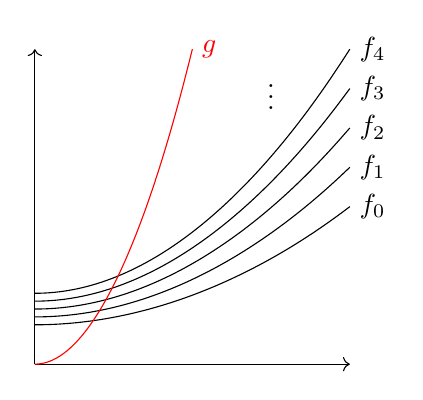
\begin{tikzpicture}
\draw[->] (0,0) -- (0,4);
\draw[->] (0,0) -- (4,0);
\draw (0,0.5) parabola bend (0,0.5) (4,2) node[right] {$f_0$};
\draw (0,0.6) parabola bend (0,0.6) (4,2.5) node[right] {$f_1$};
\draw (0,0.7) parabola bend (0,0.7) (4,3) node[right] {$f_2$};
\draw (0,0.8) parabola bend (0,0.8) (4,3.5) node[right] {$f_3$};
\draw (0,0.9) parabola bend (0,0.9) (4,4) node[right] {$f_4$};
\node at (3,3.5) {$\vdots$};
\draw[red] (0,0) parabola bend (0,0) (2,4) node[right] {$g$};
\end{tikzpicture}
\]


そしてbounding number $\mathbf{b}$を
\[
\mathbf{b} = \min \{ \kappa : \neg \B(\kappa) \}
\]
により定める.
\end{defi*}
\end{framed}

\begin{framed}
\begin{thm*}
$\kappa$を基数とするとき,$\MON(\kappa)$ならば$\B(\kappa)$かつ$\BW(\kappa)$.
したがって,$\mathbf{mon} \le \min\{\mathbf{b}, \mathbf{bw}\}$.
\end{thm*}
\end{framed}
\begin{proof}
$\MON(\kappa) \Rightarrow \BW(\kappa)$は既に示した.
そこで$\MON(\kappa) \Rightarrow \B(\kappa)$を示す.

$\mathcal{F} \subset {}^\omega \omega, |\mathcal{F}| = \kappa$とする.このとき$g: \omega \to \omega$が存在して$\forall f \in \mathcal{F}\ f \le^\ast g$を示せばよい.

一般性を失うことなく,$\forall f \in \mathcal{F}\ f(0) = 0 \land \text{$f$は狭義単調増加}$と仮定してよい.

各$f \in \mathcal{F}$について$\Psi(f): \omega \to \omega$を次で定める.
$[f(n), f(n+1))$の形の区間を考える.
$\Psi(f)$はこの形の区間上で単調減少かつ,またこの形の区間で今考えている区間の左にあるものの上の値より大きな値をとるようにする.

\[
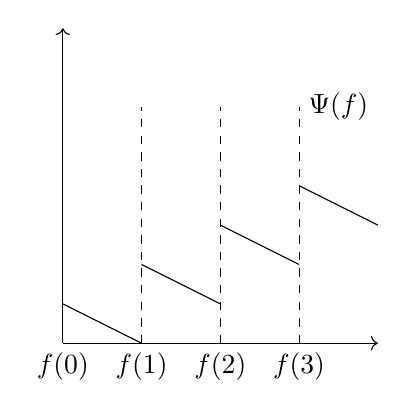
\begin{tikzpicture}
\draw[->] (0,0) -- (0,4);
\draw[->] (0,0) -- (4,0);
\draw (0,0.5) -- (1,0);
\draw (1,1) -- (2,0.5);
\draw (2,1.5) -- (3,1);
\draw (3,2) -- (4,1.5);
\draw[dashed] (1,0) -- (1,3);
\draw[dashed] (2,0) -- (2,3);
\draw[dashed] (3,0) -- (3,3);

\node[below] at (0,0) {$f(0)$};
\node[below] at (1,0) {$f(1)$};
\node[below] at (2,0) {$f(2)$};
\node[below] at (3,0) {$f(3)$};
\node at (3.5,3) {$\Psi(f)$};
\end{tikzpicture}
\]

さて,$\MON(\kappa)$を$(\Psi(f) : f \in \mathcal{F})$に適用する.
すると無限な$A \subset \omega$があって,任意の$f \in \mathcal{F}$について$(\Psi(f)(n) : n \in A)$はゆくゆくは単調である.しかし$\Psi(f)$の定め方より単調減少はありえないのでこれは単調増大になっている.
また,各$f \in \mathcal{F}$について,有限個を除くすべての$n$で$A \cap [f(n), f(n+1))$はたかだか1点である.

$g: \omega \to \omega$を次で定義する.すなわち$n\in \omega$について$g(n)$を$A$の元を昇順に並べたときの$2n$番目の元とする.
すると任意の$f \in \mathcal{F}$に対して有限個を除いた$n$について$k$があって
\[
g(n) < f(k) < f(k+1) \le g(n+1)
\]
を満たす.これは$f \le^\ast g$を導く.
\end{proof}

この定理の逆向きも示すことができるが,それは本稿では第5節の内容の帰結として得ることにする.

\section{splitting number $\mathbf{s}$と等式$\mathbf{s} = \mathbf{bw}$}


\begin{framed}
\begin{defi*}
$X, A \subset \omega$を無限集合とする.
$A$が$X$をsplitするとは$X \cap A$と$X \setminus A$がともに無限集合となることを言う.
$\mathcal{A} \subset \mathcal{P}(\omega)$がsplitting familyであるとは,どんな無限集合$X \subset \omega$についても$A \in \mathcal{A}$が存在して$A$が$X$をsplitすることである.

$\mathbf{s} = \min \{|\mathcal{F}| : \text{$\mathcal{F}$はsplitting family} \}$とおき,$\mathbf{s}$をsplitting numberという.
\end{defi*}
\end{framed}

$\mathbf{s}$と$\mathbf{bw}$について次が知られている.

\begin{framed}
\begin{thm*}
$\mathbf{s} = \mathbf{bw}$.
\end{thm*}
\end{framed}
\begin{proof}[略証]
$\mathbf{bw}$の定義において「実数」を「$\{0, 1\}$の元」に直したものは一つの基数を定めるが,それが$\mathbf{s}$と等しいことは直ちにわかる.
よって,$\mathbf{bw} \le \mathbf{s}$である.
逆向きについて.有界な実数列たちが与えられたとき,それらの$2$進小数表示の第$k$桁目を考えてそれを並べる.
実数列が収束するためには,すべての$k$についてそれらの第$k$桁目たちが収束することが十分なので,$\mathbf{s} \le \mathbf{bw}$が言える.
\end{proof}

\section{partition number $\mathbf{par}$と等式$\mathbf{par} = \mathbf{mon}$}

partition numberはラムゼーの定理のある方向での一般化がどこまで広げられるかを表す基数である.

\begin{framed}
\begin{defi*}
集合$A$に対して,$[A]^2$という記号で$A$の$2$元部分集合全体を表す.

$f: [\omega]^2 \to 2$について無限集合$A \subset \omega$が$f$についてほとんど均質集合であるとは,ある有限集合$F \subset A$があって,$f \upharpoonright [A \setminus F]^2$が定数関数となることを言う.

基数$\kappa$に対して
\[
\operatorname{R}(\kappa) \iff \begin{aligned}
&\text{任意の$(f_\alpha : \alpha < \kappa)$であって,各$f_\alpha: [\omega]^2 \to 2$とする.} \\
&\text{このとき無限集合$A \subset \omega$があって,} \\
&\text{すべての$f_\alpha$に対してほとんど均質的なものが存在する.}
\end{aligned}
\]
と定める.そしてpartition number $\mathbf{par}$を
\[
\mathbf{par} = \min \{ \kappa : \neg \operatorname{R}(\kappa) \}
\]
により定める.
\end{defi*}
\end{framed}

\begin{framed}
\begin{thm*}
$\mathbf{par} \le \mathbf{mon}$.
\end{thm*}
\end{framed}
\begin{proof}
$\operatorname{R}(\kappa)$を仮定して$\MON(\kappa)$を示せばよい.
$(f_\alpha : \alpha < \kappa)$で各$f_\alpha : \omega \to \R$なものが与えられたとする.
このとき$g_\alpha$を
\[
\begin{array}{r@{\,\,}c@{\,\,}c@{\,\,}c}
g_\alpha\colon&[\omega]^2&\longrightarrow&2\\
&\rotatebox{90}{$\in$}&&\rotatebox{90}{$\in$}\\
&\{m < n\}&\longmapsto&\begin{cases} 1 & (\text{if $f_\alpha(m) < f_\alpha(n)$}) \\ 0 & (\text{otherwise}) \end{cases}
\end{array}
\]
で定める.$(g_\alpha : \alpha < \kappa)$に$\operatorname{R}(\kappa)$を適用すると$A \subset \omega$と各$\alpha < \kappa$に対して有限集合$F_\alpha \subset A$があって,,$g_\alpha \upharpoonright [A\setminus F_\alpha]^2$が定数関数になる.
これは$f_\alpha \upharpoonright A$がゆくゆく単調になることを含意する,.
\end{proof}

今まで証明してきた事実より
\[
\mathbf{par} \le \mathbf{mon} \le \min\{\mathbf{b}, \mathbf{bw}\} = \min\{\mathbf{b}, \mathbf{s}\}
\]
である.
実は,最左辺$\mathbf{par}$と最右辺$\min\{\mathbf{b}, \mathbf{s}\}$が等しいことが証明でき,結果として上の不等式はすべて等号になる.そこで次を示そう.


\begin{framed}
\begin{thm*}
$\min\{\mathbf{b}, \mathbf{s}\} \le \mathbf{par}$.
\end{thm*}
\end{framed}
\begin{proof}
$\kappa < \min\{\mathbf{b}, \mathbf{s}\}$と仮定する.このとき$\operatorname{R}(\kappa)$を示せばよい.
$(f_\alpha : \alpha < \kappa)$で各$f_\alpha : [\omega]^2 \to 2$なものが与えられたとする.
$f_\alpha$すべてに対してほとんど均質的な無限集合を見つければよい.

まず,
\[
\begin{array}{r@{\,\,}c@{\,\,}c@{\,\,}c}
f_{\alpha,n}\colon&\omega&\longrightarrow&2\\
&\rotatebox{90}{$\in$}&&\rotatebox{90}{$\in$}\\
&x&\longmapsto&f_\alpha(\{n, x\})
\end{array}
\]
とおく.$f_{\alpha,n}$たちの個数は$\kappa \times \omega < \mathbf{s}$なので無限な$A \subset \omega$があり,$f_{\alpha,n} \upharpoonright A$たちはゆくゆくは定数である.
そこで,すべての$x \ge g_{\alpha}(n)$で$x \in A$なものについて$f_{\alpha, n}(x) = j_\alpha(n)$とする.

さらに$j_\alpha$たちの個数は$\kappa < \mathbf{s}$なので無限な$B \subset A$があって$j_\alpha \upharpoonright B$はすべてゆくゆくは定数である.
そこで,すべての$n \ge b_\alpha$で$n \in B$なものについて$j_\alpha(n) = i_\alpha$としよう.

また,$\kappa < \mathbf{b}$なので関数$h: \omega \to \omega$があって,各$\alpha < \kappa$について自然数$c_\alpha$があって$c_\alpha$以上のところで$g_\alpha$は$h$で抑えられる.

$H = \{x_0 < x_1 < \dots \}$を$B$の無限部分集合で,すべての$n$で$h(x_n) < x_{n+1}$なものとする.

これが求めるべきほとんど均質集合である.
実際,$x <  y$が$H$の元でかつ$c_\alpha, d_\alpha$より大きいものとする.
このとき,$y > h(x) \ge g_\alpha(x)$でかつ,$f_\alpha(\{x, y\}) = f_{\alpha, x}(y) = j_\alpha(x) = i_\alpha$となる.
\end{proof}


\begin{framed}
\begin{cor*}
$\mathbf{par} = \mathbf{mon} = \min\{\mathbf{b}, \mathbf{bw}\} = \min\{\mathbf{b}, \mathbf{s}\}$.
\end{cor*}
\end{framed}

\section{まとめ}

以上で出てきた$\mathbf{bw}(=\mathbf{s}), \mathbf{mon}(=\mathbf{par}), \mathbf{b}$のような実数の構造により定まる基数を基数不変量という.
$\mathbf{bw}$や$\mathbf{mon}$は有名なものではないが,それらを有名でよく調べられている基数$\mathbf{s}, \mathbf{par}$に等しいことが示せた.

基数不変量は集合論の無限組み合わせ論という分野で研究されており,位相空間論や測度論といったいわゆる普通の数学とも接していて面白い研究対象である.


\nocite{*}
\printbibliography[title=参考文献]

\end{document}